\documentclass[11pt]{article} 

\usepackage{amsmath} % required for math fuctnions
\usepackage{amssymb}
\usepackage{amsthm}
\usepackage{array} % used for table formatting
\usepackage{caption}
\usepackage{color}
\usepackage{colortbl}
\usepackage{enumitem} % used for item seperation
\usepackage{float} % used for placing float object
\usepackage{geometry} % used for page size and margins
\usepackage{graphicx} % used for graphics and figures
\usepackage{hyperref} % used for hyperlinks
\usepackage{makecell}
\usepackage{mdframed}   % For figure borders
%\usepackage{minted}
\usepackage{multirow}
\usepackage{ninecolors} % used for various colors in the specturm
\usepackage{outlines}
\usepackage{pdfcomment}
\usepackage{proposal}
\usepackage{tabularray}
\usepackage{textcomp}
\usepackage{tikz} % used to tabular array
\usetikzlibrary{arrows.meta,calc} % This is for tikzlibrat
% \usepackage[colorinlistoftodos]{todonotes}
\usepackage{soul}
\usepackage{vmargin}
\usepackage{wrapfig}
%\usepackage[table]{xcolor} 


\hypersetup{colorlinks=true,linkcolor=blue,urlcolor=blue}
\UseTblrLibrary{booktabs}
\usetikzlibrary{arrows, arrows.meta, backgrounds, fit, positioning, shapes, shapes.geometric}
\newtheorem{theorem}{Theorem}[section]
\newtheorem{lemma}[theorem]{Lemma}
 % for colors in the document and dvipsnames gives access to 68 colors
 % https://www.overleaf.com/learn/latex/Using_colors_in_LaTeX
\setpapersize{USletter} % Set paper and margins
\setmarginsrb{1in}{1in}{1in}{1in}{0pt}{0mm}{0pt}{0mm}

\title{
    \vspace{-45pt}
    \fontsize{15pt}{18pt}\selectfont
    \textcolor{FlyersRed}
    {\textbf{POSE Phase I}: Enabling an Open Ecosystem for Thermo-Fluid Computational Intelligence in Manufacturing and Energy Systems}
}
\date{}
\author{}


% Define M column type
\newcolumntype{M}[1]{>{\centering\arraybackslash}m{#1}}
\newcolumntype{R}[1]{>{\raggedleft\arraybackslash}m{#1}}

\newcommand{\CO}[1]{CO\textsubscript{#1}}




\begin{document}
\pagestyle{empty} % To remove page nubering
% \pagenumbering{gobble} % NO page numbers for research.gov
\vspace{-4\baselineskip}
\begin{center}
    \Large\textbf{\textcolor{FlyersRed}{PROJECT SUMMARY}}
\end{center}
\vspace{-1.4\baselineskip}


\section*{Overview}
\vspace{-3pt}
\noindent
This Phase-I research aims at a structured transition of FAME (https://github.com/neoceph/FAME), a machine learning (ML) augmented finite-volume based thermal CFD solver, into a sustainable, distributed Open-Source Ecosystem (OSE) for Additive Manufacturing (AM) and supercritical (s\CO{2})  researchers. FAME is available to researchers under an open-source license on GitHub and has been validated against NIST metal AM experiments1, attracting limited academic research users. The proposed OSE will provide targeted training and illustrative use cases, covering topics such as the design and analysis of AM processes and the production of s\CO{2}-based energy systems. Phase I activities will include: 1) formalizing the managing organization; 2) developing an effective governance model; 3) identifying and expanding the external developer and user community; and 4) designing the onboarding, outreach, licensing, and sustainability strategies for tool support. Tool development and support are led by Dr. Abdullah A. Amin and Dr. Andrew J. Schrader from the Mechanical and Aerospace Engineering Department at the University of Dayton. These researchers bring domain expertise in the design, optimization, and application of AM and Energy Systems, directly responding to the broader need for open, reproducible, and extensible infrastructure in manufacturing and energy research and development. This proposal focuses on building the foundation for a sustainable and community-driven OSE for manufacturing and energy research.
%
\vspace{-3pt}
\section*{Intellectual Merit}
\vspace{-3pt}
\noindent
This project will advance the FAME framework into a sustainable, community-driven open-source ecosystem (OSE) that supports high-fidelity thermal-fluid simulations for additive manufacturing (AM) and s\CO{2}-based thermal management. Emphasizing reproducibility, modularity, and extensibility, FAME integrates data-augmented modeling with ray-tracing-based radiative heat transfer to accurately capture beam-powder interactions and phase change dynamics key to understanding defect formation, microstructure evolution, and thermal system performance. Designed for heterogeneous CPU/GPU architectures, the framework supports scalable simulations and enables rapid iteration. By coupling physics-based solvers with modern ML libraries, it provides a rigorous platform to develop and validate AI/ML methods for surrogate modeling, real-time optimization, and intelligent process control. The project will formalize a flexible architectural design and foster a distributed contributor base to sustain long-term innovation. Integrated training resources will support the onboarding of new users, reducing entry barriers while enabling participation in advancing computational methods for intelligent manufacturing and energy systems \cite{aminComputationalHomogenizationElastic2018,aminHighThroughputParticle2014,aminMechanicalAnalysisMgB22017,aminMultiscaleMultiphysicsModel2016,aminMULTISCALEMULTIPHYSICSTHERMOMECHANICAL2018}.
\vspace{-3pt}
\section*{Broader Impacts}
\vspace{-3pt}
\noindent
The FAME OSE ecosystem will democritize access to advanced thermal-fluid simulation and AI-assisted design tools across the manufacturing and energy sectors. A central aim is to train the next generation of researchers, engineers, and developers in open-source software development, digital twin technologies, and thermo-fluid modeling specific to manufacturing and energy. The project will offer annual hands-on workshops and summer schools focused on software sustainability and domain-specific applications. A targeted talent development initiative will engage institutions across various geographic regions through customized outreach and curriculum modules, helping to prepare a skilled, workforce-ready STEM pipeline. Research outcomes and practical use cases will be shared through peer-reviewed publications, conference tutorials, and freely accessible training materials hosted on the project's online platform and amplified through social media. By fostering a community grounded in open science, reproducibility, and collaborative development, this initiative will advance U.S. priorities in energy and manufacturing while ensuring the long-term sustainability of the FAME platform.

\newpage 
% \vspace*{-10pt}
\maketitle
\thispagestyle{empty} % No page numbers
\vspace{-45pt}
\section{Research Motivation and Objectives}
\label{sec:intro}
% \todo{Overview figure needs to be changed.}

\begin{wrapfigure}[19]{r}{0.5\textwidth} % 'r' for right, width is adjustable
	\vspace{-20pt} % Optional: adjust vertical position
	\centering
	\begin{mdframed}[roundcorner=5pt, linewidth=0pt, innerleftmargin=-0pt, innerrightmargin=0pt]
		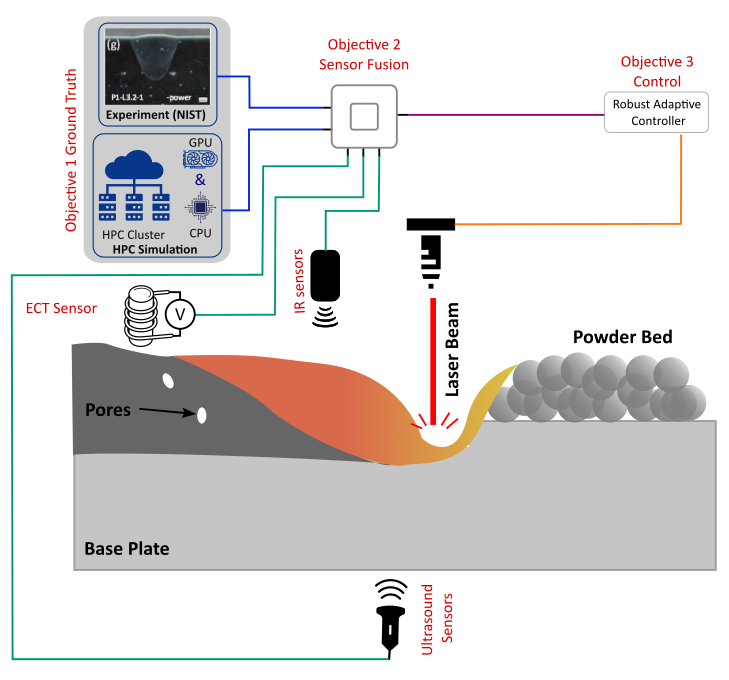
\includegraphics[width=0.99\textwidth]{./figures/SensorFusion.png}
	\end{mdframed}
	\vspace{-24pt}   % Vertical space after the figure
	\caption{\emph{Dummy figure as an example.}}
    \pdfcomment[icon=Note, color=FlyersRed, open=true]{This figure is a placeholder and needs to be updated based on proposal.}
	\label{fig:sensor-fusion}
	\vspace{-10pt}  % Additional space after caption
\end{wrapfigure}

In a usual template I prefer writing some words about motivation as to why we want to do this and what are the objective in terms of scientific outcome. NSF is about fundamental research and they prefer hypothesis driven activities. Although for the NSF POSE, this might be different. If we need to cite anything, we do this by \cite{aminPhysicsGuidedHeat2024} By the end of the paragraph, I want to spell out the \textbf{scientific understanding} in terms of bulleted lists:


\vspace{-10pt}
\begin{itemize}[label=\textbullet, align=left, labelwidth=4em, labelsep=1em, leftmargin=*,noitemsep]
    \item \textbf{Understanding 1:} What new understanding we want to develop.
    \item \textbf{Understanding 2:} Any additional understanding?
    \item \textbf{Understanding 3:} Anything else that we missed?
\end{itemize}

\vspace{-10pt}
In terms of novelty, what novel \textbf{novel scientific outcomes} will results as part of this fundamental research:

\vspace{-10pt}
\begin{itemize}[label=\textbullet, align=left, labelwidth=4em, labelsep=1em, leftmargin=*,noitemsep]
    \item We will have a growing developer and user base of machine learning based thermal CFD solver.
    \item The framework is highly flexible and application agnostic.
    \item Anything else.
\end{itemize}


\begin{dashtcb}[FlyersBlue]{Research Goal}[width=\linewidth]
We use textbox to highlight the research goal of the proposal.
\end{dashtcb}

\begin{dashtcb}[FlyersRed]{Educational Goal}[width=\linewidth]
	Do the same for educational goal of the proposal.
\end{dashtcb}

\section{Background and State of the Art}
\label{sec:background}

Not sure if this is appropriate for the POSE proposal.

\subsection{Subsection 1}
\label{sec:subsection1}

Text description

\begin{table}[H]
	\renewcommand{\arraystretch}{1.8}
	\centering
	\caption{\emph{Example table that may contain multiple rows and columns. This is a dummy table to show how to use the table environment.}}
	\vspace{-10pt}
	\label{tbl:table1}
	\begin{tikzpicture}
		% Draw the table
		\node (tbl) at (0,0) {
			\begin{tabular}{R{0.19\textwidth} M{0.25\textwidth} M{0.22\textwidth} M{0.20\textwidth}}
				\rowcolor{azure8}
				Item 1 & Item 2 & Item 3 & Item 4 \\
				row 11 & row 12 & row 13 & row 14 \\
				row 21 & row 22 & row 23 & row 24 \\
				row 31 & row 32 & row 33 & row 34 \\
				row 41 & row 42 & row 43 & row 44 \\
				row 51 & row 52 & row 53 & row 54 \\
				row 61 & row 62 & row 63 & row 64 \\
				row 71 & row 72 & row 73 & row 74 \\
				row 81 & row 82 & row 83 & row 84 \\
				row 91 & row 92 & row 93 & row 94 \\
			\end{tabular}
		};
		
		% Draw the arrow aligned to the table height
		\draw[very thick, ->, >=latex] (-7.45,2.7) -- (-7.45,-3.3);
		\node[rotate=90] at (-7.75, -0.3) {\small If arrow needed};
	\end{tikzpicture}
\end{table}

\subsection{Subsection 2}
\label{sec:subsection2}

More texts

\subsection{Subsection 3}
\label{sec:subsection3}

More texts

\section{Proposed Research Approach}
Proposed research approach or research activities that aligns with POSE

%\noindent
%\textbf{Expected Scientific Outcomes:}
\vspace{-10pt}
\begin{enumerate}[label=\textbf{Objective-\arabic*:}, align=left, labelwidth=4em, labelsep=1em, leftmargin=*,noitemsep]
    \item Item 1 with \textbf{sufficient highlights to ensure that the reader does not miss important key details} as there is always a chance for the panel reviewer to misunderstand the objective.
    \item Another key \textbf{objective} to achieve the final goal.
    \item Another key \textbf{aspect of the proposed} activitied.
\end{enumerate}

\begin{figure}[htbp]
	\centering
	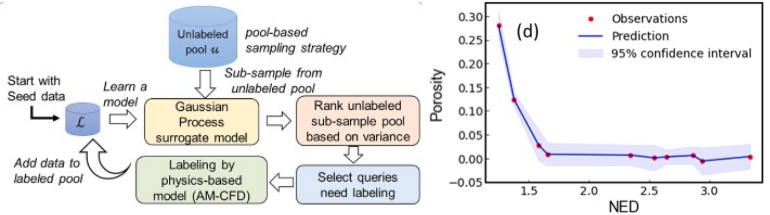
\includegraphics[width=0.95\textwidth]{./figures/ActiveLearning.png} % Replace with your image
    \vspace{-13pt}  % Additional space after caption
    \caption{\emph{Another example image with citation \cite{mojumderLinkingProcessParameters2023}.}}
	\label{fig:active-learning}
    \vspace{-20pt}  % Additional space after caption
\end{figure}
%
%\vspace{-20pt}
\section{Objectives}
\label{sec:objectives}
\subsection{Objective-1: (Amin)}
\label{sec:object1}


\noindent
\textbf{\textcolor{FlyersRed}{{Goal:}}}
\textit{Specify the goal.}



\noindent
\textbf{\textcolor{FlyersRed}{{Proposed Approach:}}}
Proposed approach description.

\noindent
\textbf{\textcolor{FlyersRed}{{Mitigation:}}}
Mitigation plan if any.


\textbf{\textcolor{FlyersRed}{{Expected Outcome:}}}
Explain expected outcome. 

%\vspace{-20pt}
\section{Objectives}
\label{sec:objectives}
\subsection{Objective-1: (Amin)}
\label{sec:object1}


\noindent
\textbf{\textcolor{FlyersRed}{{Goal:}}}
\textit{Specify the goal.}



\noindent
\textbf{\textcolor{FlyersRed}{{Proposed Approach:}}}
Proposed approach description.

\noindent
\textbf{\textcolor{FlyersRed}{{Mitigation:}}}
Mitigation plan if any.


\textbf{\textcolor{FlyersRed}{{Expected Outcome:}}}
Explain expected outcome. 

\begin{equation}\label{eq:example_equation}
  m_{1\oplus...n}(C) 
  = \frac{1}{1 - K} \sum_{\substack{A_1 \cap A_2 ... \cap A_n = C}} m_1(A_1)\,...m_n(A_n),
  \quad
  K = \sum_{\substack{A_1 \cap A_2 ... \cap A_n = \varnothing}} m_1(A_1)\,...m_n(A_n)
\end{equation}

\noindent where: $m_1(A_1)$ and $m_n(A_n)$ are the basic belief assignments from source 1 (transformer sensor 1) and source n (transformer sensor n) for propositions $A_1, ... A_n \subseteq \Theta$; $m_{1\oplus...n}(C)$ is the fused belief mass for proposition $C \subseteq \Theta$; $K$ is the conflict mass representing total evidence conflict among $m_1$, ... $m_n$; $A_1, .., A_n$ are subsets of the frame of discernment $\Theta$ describing melt-pool regimes (insufficient, nominal, keyhole, lack\_of\_fusion) extending sequentially across all sources. From the fused mass function $m_{DS}(\cdot)$ we compute belief $\mathrm{Bel}(\text{``nominal''})$ and plausibility $\mathrm{Pl}(\text{``nominal''})$ their interval width $\mathrm{Pl}-\mathrm{Bel}$ serves as an explicit uncertainty metric.

%\vspace{-20pt}
\section{Objectives}
\label{sec:objectives}
\subsection{Objective-3: (Amin)}
\label{sec:object3}


\noindent
\textbf{\textcolor{FlyersRed}{{Goal:}}}
\textit{Specify the goal.}



\noindent
\textbf{\textcolor{FlyersRed}{{Proposed Approach:}}}
Proposed approach description.

\noindent
\textbf{\textcolor{FlyersRed}{{Mitigation:}}}
Mitigation plan if any.


\textbf{\textcolor{FlyersRed}{{Expected Outcome:}}}
Explain expected outcome. 


\section{Intellectual Merit}
This project will advance the FAME framework into a sustainable, community-driven open-source ecosystem (OSE) that supports high-fidelity thermal-fluid simulations for additive manufacturing (AM) and s\CO{2}-based thermal management. Emphasizing reproducibility, modularity, and extensibility, FAME integrates data-augmented modeling with ray-tracing-based radiative heat transfer to accurately capture beam-powder interactions and phase change dynamics key to understanding defect formation, microstructure evolution, and thermal system performance. Designed for heterogeneous CPU/GPU architectures, the framework supports scalable simulations and enables rapid iteration. By coupling physics-based solvers with modern ML libraries, it provides a rigorous platform to develop and validate AI/ML methods for surrogate modeling, real-time optimization, and intelligent process control. The project will formalize a flexible architectural design and foster a distributed contributor base to sustain long-term innovation. Integrated training resources will support the onboarding of new users, reducing entry barriers while enabling participation in advancing computational methods for intelligent manufacturing and energy systems.
 
\section{Outreach Plan}  
\subsection{Community Outreach} 
Detailing out the plan

\subsection{Student Involvement}  
Discuss student involvement

\subsection{Curriculum Development}  
Do we want to develop any curriculum for this project? If yes, then what is the plan?

\subsection{Dissemination through Conferences}  
How dow we want to disseminate the research outcomes? Do we have any plan to present at conferences through workshop and attract more developers?

\section{Broader Impacts}
The FAME OSE ecosystem will democritize access to advanced thermal-fluid simulation and AI-assisted design tools across the manufacturing and energy sectors. A central aim is to train the next generation of researchers, engineers, and developers in open-source software development, digital twin technologies, and thermo-fluid modeling specific to manufacturing and energy. The project will offer annual hands-on workshops and summer schools focused on software sustainability and domain-specific applications. A targeted talent development initiative will engage institutions across various geographic regions through customized outreach and curriculum modules, helping to prepare a skilled, workforce-ready STEM pipeline. Research outcomes and practical use cases will be shared through peer-reviewed publications, conference tutorials, and freely accessible training materials hosted on the project's online platform and amplified through social media. By fostering a community grounded in open science, reproducibility, and collaborative development, this initiative will advance U.S. priorities in energy and manufacturing while ensuring the long-term sustainability of the FAME platform.

\section{Project Timeline}
	\begin{table}[h]
	\centering
	\caption{A Tentative project timeline}
	\begin{tblr}{
			colspec = {X[0.75,c,m]},
			row{1-6} = {font=\bfseries},
			row{3} = {bg=purple8,fg=black,font=\bfseries}, % This allows you customize the colors for each row
			row{4} = {bg=azure9,fg=black,font=\bfseries},
			row{5} = {bg=brown8,fg=black,font=\bfseries},
			hlines = 1.5pt, vlines = 1.5pt % You can customize the size of hlines and vlines
%			hline{3,4} = {dashed,fg=gray}, % This is another type of customization for hlines to be dashed gray
		}
		\SetCell[r=2]{c} {Research\\Plan} & \SetCell[c=4]{c} Year 1 & & & & \SetCell[c=4]{c} Year 2 & & & & \SetCell[c=4]{c} Year 3 & & & \\
		& Q1 & Q2 & Q3 & Q4 & Q1 & Q2 & Q3 & Q4 & Q1 & Q2 & Q3 & Q4 \\
		Objective -1 & \SetCell[c=4]{} 
		
\begin{tikzpicture}[overlay, remember picture]
			\draw[line width=1mm, double, {Stealth[length=6mm]-Stealth[length=6mm]}] (0,0.1) to ++(3.5,0);
		\end{tikzpicture}  & & & & & & & & & \\
		
		Objective -2 & & & & \SetCell[c=4]{} 
		
\begin{tikzpicture}[overlay, remember picture]
			\draw[line width=1mm, double, {Stealth[length=6mm]-Stealth[length=6mm]}] (0,0.1) to ++(3.5,0);
		\end{tikzpicture} & & & & & & & & \\
		Objective -3 & & & & & & & & \SetCell[c=4]{} 
		
\begin{tikzpicture}[overlay, remember picture]
			\draw[line width=1mm, double, {Stealth[length=6mm]-Stealth[length=6mm]}] (0,0.1) to ++(3.5,0);
		\end{tikzpicture} & & & & \\
		Objective -4 & & \SetCell[c=3]{} 
		
\begin{tikzpicture}[overlay, remember picture]
			\draw[line width=1mm, double, {Stealth[length=6mm]-Stealth[length=6mm]}] (0,0.1) to ++(2.5,0);
		\end{tikzpicture} & & & & & \SetCell[c=4]{} 
		
\begin{tikzpicture}[overlay, remember picture]
			\draw[line width=1mm, double, {Stealth[length=6mm]-Stealth[length=6mm]}] (0,0.1) to ++(3.8,0);
		\end{tikzpicture} & & & & & \\
		{Education \& Outreach} & \SetCell[c=4]{c} {Conference?}  & & & &  \SetCell[c=4]{c} {XXX \\ workshop}  & & & & \SetCell[c=4]{c} {Dayton STEM \\ workshop}  & & & \\
        Dissemination & \SetCell[c=4]{c} {Conference XXX}  & & & &  \SetCell[c=4]{c} {Conference}  & & & & \SetCell[c=4]{c} {Conference \\ shortcourse}  & & & \\
	\end{tblr}
\end{table}

\section{Prior NSF Support}
The PI's have no prior NSF support.
\newpage
\bibliographystyle{unsrt}
\bibliography{reference}
\end{document}